\documentclass[20pt]{article}
\usepackage{graphicx}
\setlength\parindent{0pt}
\usepackage{amsfonts}
\usepackage{courier}
\begin{document}
\title{Soundcool's Meter Sub-module Specification}
\maketitle

This is a specification for meter sub-module used in many soundcool modules to visualize audio level in decibels.
\section*{User interface}
Meter is used in various soundcool modules. For instance:

%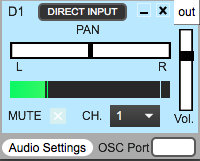
\includegraphics[scale=0.5]{directin.png} 
%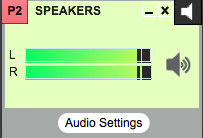
\includegraphics[scale=0.5]{speakers.png} 

\begin{figure}[htp]

\centering
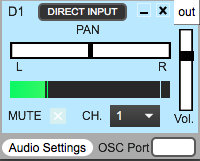
\includegraphics[scale=0.5]{directin.png} 
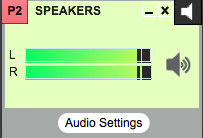
\includegraphics[scale=0.5]{speakers.png} 
\caption{Direct Input and Speakers modules (from left to right)}
\label{fig:figure3}
\end{figure}

\section*{Web Audio Implementation}
Decibels (dB) is a relative measure of loudness. A useful dB measurement Decibels relative to Full Scale (dBFS) is anchored on the maximum peak level possible in a system. In Web Audio, this peak level is \texttt{1}. Perceived loudness and amplitude of the wave share an exponential relationship:

\begin{equation}
dB = 20 * log_{10}(a / a_{0})
\end{equation}
where \texttt{a} is the amplitude of the wave and $a_0$ is the peak amplitude.
So equation (1) reduces to:
\begin{equation}
dB = 20 * log_{10}(a)
\end{equation}
Amplitude of the wave (\texttt{a} in equation above) is calculated by computing the root mean square (RMS) of a buffer of audio sample's time domain data.
\begin{equation}
a = \sqrt{\frac{\sum_{i=1}^{n}x_i^2}{n}}
\end{equation} 
where $x_i$ is a float \texttt{number} in the range [-1, 1] when there is no clipping. \texttt{n} is the length of the array set to 256.\\
\\
So, the resulting range in decibels (dB) for an unclipped signals is [-$\infty$, 0] since RMS ranges from [0, 1]. 

\section*{References}
\begin{itemize}
\item http://teropa.info/blog/2016/08/30/amplitude-and-loudness.html
\end{itemize}


\end{document}